%%%%%%%%%%%%%%%%%%%%%%
% NASTAVENÍ FEKT.TEX %
%%%%%%%%%%%%%%%%%%%%%%

% Pokud následující řádky zakomentujete, na titulní straně se nezobrazí.

% Nadpis dokumentu (kód předmětu)
\newcommand{\name}{FEKT.tex}
% Podnadpis dokumentu (název předmětu)
%\newcommand{\subname}{}
% Seznam autorů
\newcommand{\authors}{Studenti IBE}
% Seznam korektorů
%\newcommand{\corrections}{}
% Popis dokumentu
\newcommand{\docdesc}{Univerzální šablona pro~český text}
% Zařazení dokumentu (studijní program)
\newcommand{\docgroup}{Informační bezpečnost, FEKT VUT}
% Odkaz
\newcommand{\docurl}{https://github.com/VUT-FEKT-IBE/FEKT.tex}

% Přepsáním argumentu na 'true' zapnete balíček 'minted' pro sázení kódu.
% Pro jeho použití lokálně musíte mít v systému dostupný Python 3, python
% knihovnu 'minted' a PDFLaTeX musíte spouštět s argumentem '-shell-escape'.
% Místo něj můžete použít prostředí 'lstlisting'.
\newcommand{\docminted}{false}


%%%%%%%%%%%%%%%%%%%%
% OBECNÉ NASTAVENÍ %
%%%%%%%%%%%%%%%%%%%%

\newcommand{\fekttexversion}{2.0}

\documentclass[
    % Velikost základního písma je 12 bodů
    12pt,
    % Formát papíru je A4
    a4paper,
    % Oboustranný tisk
    twoside,
    % Záložky a metainformace ve výsledném PDF budou v kódování unicode
    unicode,
]{article}

% Kódování zdrojových souborů
\usepackage[utf8]{inputenc}
% Kódování výstupního souboru
\usepackage[T1]{fontenc}
% Podpora češtiny
\usepackage[czech]{babel}

% Geometrie stránky
\usepackage[
    % Horní a dolní okraj
    tmargin=25mm,
    bmargin=25mm,
    % Vnitřní a vnější okraj
    lmargin=30mm,
    rmargin=20mm,
    % Velikost zápatí
    footskip=17mm,
    % Vypnutí záhlaví
    nohead,
]{geometry}

% Zajištění kopírovatelnosti a prohledávanosti vytvořených PDF
\usepackage{cmap}
% Podmínky (pro použití v titulní straně)
\usepackage{ifthen}

%%%%%%%%%%%%%%%
% FORMÁTOVÁNÍ %
%%%%%%%%%%%%%%%

% Nastavení stylu nadpisů
\usepackage{sectsty}
% Formátování obsahů
\usepackage{tocloft}
\setcounter{tocdepth}{1}
% Odstranění mezer mezi řádky v seznamech
\usepackage{enumitem}
\setlist{nosep}
\setitemize{leftmargin=1em}
\setenumerate{leftmargin=1.5em}
\renewcommand{\labelitemi}{--}
\renewcommand{\labelitemii}{$\circ$}
\renewcommand{\labelitemiii}{$\cdot$}
\renewcommand{\labelitemiv}{--}
% Sázení správných uvozovek pomocí '\enquote{}'
\usepackage{csquotes}
% Vynucení umístění poznámek pod čarou vespod stránky
\usepackage[bottom]{footmisc}
% Automatické zarovnání textu k předcházení vdov a parchantů
\usepackage[defaultlines=3,all=true]{nowidow}
% Zalomení části textu pokud není na současné stránce dost místa
\usepackage{needspace}
% Nastavení řádkování
\usepackage{setspace}
\onehalfspacing
% Změna odsazení odstavců
\setlength{\parskip}{1em}
\setlength{\parindent}{0em}

% Bezpatkové sázení nadpisů
\allsectionsfont{\sffamily}
% Změna formátování nadpisu a podnadpisů v Obsahu
\renewcommand{\cfttoctitlefont}{\Large\bfseries\sffamily}
\renewcommand{\cftsubsecdotsep}{\cftdotsep}

% Použití moderní/aktualizované sady písem
\usepackage{lmodern}

%%%%%%%%%%%
% NADPISY %
%%%%%%%%%%%

\usepackage{titlesec}

\titlespacing*{\section}{0pt}{10pt}{-0.2\baselineskip}
\titlespacing*{\subsection}{0pt}{0.2\baselineskip}{-0.2\baselineskip}
\titlespacing*{\subsubsection}{0pt}{0.2\baselineskip}{-0.2\baselineskip}
\titlespacing*{\paragraph}{0pt}{0pt}{1em}

%%%%%%%%%%
% ODKAZY %
%%%%%%%%%%

% Tvorba hypertextových odkazů
\usepackage[
    breaklinks=true,
    hypertexnames=false,
]{hyperref}
% Nastavení barvení odkazů
\hypersetup{
    colorlinks,
    citecolor=black,
    filecolor=black,
    linkcolor=black,
    urlcolor=blue
}

%%%%%%%%%%%%%%%%%%%%%%%%%%%
% OBRÁZKY, GRAFY, TABULKY %
%%%%%%%%%%%%%%%%%%%%%%%%%%%

% Vkládání obrázků
\usepackage{graphicx}
\usepackage{subfig}
% Nastavení popisů obrázků, výpisů a tabulek
\usepackage{caption}
\captionsetup{justification=centering}
% Grafy a vektorové obrázky
\usepackage{tikz}
\usetikzlibrary{shapes,arrows}
% Složitější tabulky
\usepackage{tabularx}
\usepackage{multicol}

% Sázení osamocených float prostředí v horní části stránky
\makeatletter
\setlength{\@fptop}{0pt plus 10pt minus 0pt}
\makeatother

% Vynucení vypsání floating prostředí pomocí \FloatBarrier
\usepackage{placeins}

% Rámečky
\usepackage{mdframed}

%%%%%%%%%%%%%%
% MATEMATIKA %
%%%%%%%%%%%%%%

% Sázení matematiky a matematických symbolů ('\mathbb{}')
\usepackage{amsmath}
\usepackage{amssymb}
% Sázení fyzikálních veličin
\usepackage{siunitx}

%%%%%%%%%%%%%%%%%
% ZDROJOVÉ KÓDY %
%%%%%%%%%%%%%%%%%

% Sazba zdrojových kódů
\usepackage[formats]{listings}
% Přepnutí prostředí 'code' do režimu výpisu kódu
\newenvironment{code}{\captionsetup{type=listing}}{}

\lstset{
    basicstyle=\small\ttfamily,
    numbers=left,
    numberstyle=\tiny,
    tabsize=4,
    columns=fixed,
    showstringspaces=false,
    showtabs=false,
    keepspaces,
}

% Balíček 'minted' budeme používat pouze pokud je jeho hodnota nastavena na 'true'
\providecommand{\docminted}{false}
\ifthenelse{\equal{\docminted}{true}}
{
    % Sazba zdrojových kódů
    \usepackage[newfloat]{minted}
    % Nastavení barev 'minted' kódů
    \usemintedstyle{pastie}
}
{
    % \docminted není 'true', nic neprovádíme
    % Pokud je v dokumentu 'minted' prostředí, dokument se nepodaří přeložit.
}

%%%%%%%%%%%%%%%%%%%
% VLASTNÍ PŘÍKAZY %
%%%%%%%%%%%%%%%%%%%

\newcounter{todo}
\newcommand{\TODO}[1]{%
    \addtocounter{todo}{1}%
    \textcolor{red}{%
    \textbf{\sffamily\small{TODO \thetodo}%
    \ifthenelse{\equal{#1}{}}{}{:}%
    } %
    #1%
    }%
}

%%%%%%%%%%%
% TITULKA %
%%%%%%%%%%%

\newcommand{\titulka}{
    \vspace*{2em}
    \begin{center}
        \ifthenelse{\isundefined{\name}}{}{{\Huge \bfseries \name{}}}

        \ifthenelse{\isundefined{\subname}}{}{{\huge \bfseries \subname{}}}

        \vspace*{2em}

        \ifthenelse{\isundefined{\docdesc}}{}{{\Large \docdesc}}

        \vspace*{1em}

        \ifthenelse{\isundefined{\docgroup}}{}{\docgroup}

        \ifthenelse{\isundefined{\docurl}}{}{\url{\docurl}}
    \end{center}

    \vfill

    \ifthenelse{\isundefined{\authors}}{}{\authors{}}
    \ifthenelse{\isundefined{\corrections}}{}{\\\small (korektury \corrections{})}

    {}{\small \today}
    \\{\small FEKT.tex \fekttexversion{}}

    \thispagestyle{empty}
    \newpage
}

%%%%%%%%%%%%
% DOKUMENT %
%%%%%%%%%%%%

\begin{document}

\titulka{}

\tableofcontents
\thispagestyle{empty}

\setcounter{page}{0}

\clearpage
\section[O~LaTeXu]{O~\LaTeX{}u}

\subsection{Co je \LaTeX}

\LaTeX{} je sázecí systém pro~tvorbu (nejen) odborných dokumentů.
Uživatel píše \emph{plain text}, který je pak dle použitých značek převeden na~výsledný dokument.
Oproti tomu programy typu Microsoft Word píšou rovnou formátovaný text, tzv. WYSIWYG (\emph{\enquote{What You See Is What You Get}}).

Hlavními výhodami \LaTeX{}u jsou především vysoká typografická kvalita, jednoduchá přenositelnost (všichni známe rozbité Word dokumenty) a jednotnost stylu (velikosti písma, typy fontů) či možnost \LaTeX{}ové dokumenty verzovat \texttt{git}em.

\subsection{LaTeX na FEKTu}

Všechny oficiální šablony pro studium na FEKTu můžete najít na~
\url{https://latex.feec.vutbr.cz/}.

Také doporučujeme předmět \href{https://www.vut.cz/studenti/predmety/detail/224331?apid=224331}{BPC-ZSG}, který je na~VUT FEKT povinně volitelný předmět programů BPC-AUD, BPC-IBE, BPC-SEE a~BPC-TLI.

\subsection{Jak na Overleaf?}

Nejdříve si z \url{https://github.com/VUT-FEKT-IBE/FEKT.tex}
stáhněte šablonu FEKT.tex (jejíž výstup právě čtete).
V~Overleaf vyberte možnost \texttt{New Project > Upload Project} a~nahrajte staženou šablonu.

Po~otevření šablony otevřete menu v~levém horním rohu v~možnosti \texttt{Main Document} a~vyberete \texttt{main.tex} nebo \texttt{text/01.tex}.
Dokument samotný pak kompilujte \emph{v~jakémkoliv aktivním \texttt{.tex} souboru} krom \texttt{shared.tex}.

Pokud chcete oddělit jednotlivé textové soubory a~vkládat je do~dokumentu zvlášť, stačí v~záložce \texttt{text} vytvořit nový soubor s~příponou \texttt{.tex}.
V~souboru \texttt{main.tex} pak daný soubor načtěte pomocí příkazu \verb|\include{file_path}|.

Dokument samotný se kompiluje pomocí tlačítka \texttt{Recompile}, případně zkratkou \texttt{Ctrl} + \texttt{Enter}.
Tlačítko pro~stažení PDF souboru se nachází vedle \texttt{Recompile}.


\clearpage
\section[Struktura LaTeXového ]{Struktura \LaTeX{}ového textu}

Pro~vytvoření \enquote{hlavního nadpisu} (jako je název kapitoly hned nad tímto odstavcem) použijeme příkaz \verb|\section{text}|.
Jednotlivé oddíly se číslují automaticky vzesupně.

Pro~vytvoření podnadpisů (třeba část \ref{sec:seznamy} níže) použijeme příkaz  \verb|\subsection{text}|.
Stejně jako hlavní nadpisy se číslují automaticky.

Nové odstavce se vytváří automaticky, pokud vynecháme jeden řádek.
Řádek jako takový můžeme také zalomit dvěma zpětnými lomítky \verb|\\|.

\begin{figure}[ht]
\onehalfspacing
\begin{mdframed}
\begin{verbatim}
V~půlce této věty řádek lámu pouze v~kódu
a~text je přesto sázen dál.
\end{verbatim}

V~půlce této věty řádek lámu pouze v~kódu
a~text je přesto sázen dál.

\begin{verbatim}
V~půlce této věty řádek lámu\\
a~text tak není sázen až do~konce, i~když pro~to prostor má.
\end{verbatim}

V~půlce této věty řádek lámu\\
a~text tak není sázen až do~konce, i~když pro~to prostor má.
\end{mdframed}
\end{figure}

Nezlomitelná mezera se píše pomocí vlnovky (\texttt{\~}): \verb|v~domě|.
Používejte ji za~všemi předložkami a~spojkami, ty na~konce řádků nepatří.

Psát ji vždy a~všude (a~ne jen když se zrovna dostane na~konec řádku z~důvodu sazby) má několik velkých výhod.
Především vám to ušetří čas: nebudete si při psaní textu hlídat jestli náhodou na~konci řádku nejste a~můžete se soustředit pouze na~obsah.
A~ušetříte tím i~čas, protože tyto tvrdé mezery nebudete muset zpětně doplňovat.

\LaTeX{}ové soubory můžete komentovat pomocí značky \verb|%|: cokoliv za~touto značkou se sázet nebude (a~textové editory podporující \LaTeX{}ovou syntaxi vám takový text barevně zvýrazní).
Můžete tak v~textu zanechávat poznámky (své zdroje, nejasnosti, TODO) aniž by byly vidět ve~finální verzi dokumentu.

\subsection{Seznamy}
\label{sec:seznamy}

Nečíslované seznamy se vytváří v~prostředí \verb|itemize|:
jednotlivé body oddělujeme značkou \verb|\item|.

Číslované seznamy fungují obdobně a~vytváří se prostředím \verb|enumerate|.
Tato dvě prostředí do~sebe lze vnořovat.

\begin{figure}[ht]
\begin{mdframed}
\onehalfspacing
\begin{verbatim}
\begin{itemize}
    \item itemize první úrovně
    \begin{itemize}
        \item itemize druhé úrovně
        \begin{enumerate}
            \item první položka enumerate
            \item druhá položka enumerate
        \end{enumerate}
    \end{itemize}
\end{itemize}
\end{verbatim}

\vspace*{1em}

\begin{itemize}
    \item itemize první úrovně
    \begin{itemize}
        \item itemize druhé úrovně
        \begin{enumerate}
            \item první položka enumerate
            \item druhá položka enumerate
        \end{enumerate}
    \end{itemize}
\end{itemize}
\end{mdframed}
\end{figure}
\FloatBarrier

Většina autorů píše stejným způsobem jako ve~Wordu, a~\enquote{Enter} v~kódu píše až na~konci odstavce.
Psát každou větu na~svůj řádek však přináší výhodu: když je kód verzován pomocí \texttt{git}u, vznikají menší \texttt{diff}y a~změny jsou lépe vidět.
Tak je strukturován i~tento dokument.
 
\subsection{Zvýraznění v~textu}

\begin{table}[ht]
\centering
\begin{tabular}{|l|l|}
značka & ukázka \\
\hline \hline
\texttt{textbf} & \textbf{tučné písmo} \\
\texttt{emph} & \emph{kurzíva} \\
\texttt{enquote} & \enquote{text v~uvozovkách} \\
\texttt{texttt} & \texttt{strojový text} \\
\texttt{underline} & \underline{podtržený text} \\
\end{tabular}
\end{table}
\FloatBarrier

Pamatujte však, že se tyto značky mají používat pouze výjimečně, protože na~sebe poutají pozornost.


\clearpage
\section{Matematika a~vzorce}

Matematika může být sázena ve~dvou režimech.

Režim \emph{inline} text sází do~řádku jako text a~je vhodný pro~menší nebo méně důležité vzorce:
$\sum_{i=0}^{10} \sin (x + \pi)$.
Text se zde uzavírá mezi značky \verb|$|.

Režim \emph{outline} lze použít naprosto stejně, ale vzorec uzavřete mezi dvojité \verb|$$|:
$$\sum_{i=0}^{10} \sin (x + \pi).$$

Pokud chcete vzorce číslovat nebo jich vypsat více za~sebou, lze použít prostředí \texttt{align}:
% Zdroj rovnic: https://latex-tutorial.com/align-equations/
\begin{align*}
f(u) & =\sum_{j=1}^{n} x_jf(u_j) \\
     & =\sum_{j=1}^{n} x_j \sum_{i=1}^{m} a_{ij}v_i \\
     & =\sum_{j=1}^{n} \sum_{i=1}^{m} a_{ij}x_jv_i
\end{align*}

\begin{table}[ht]
\centering
\begin{tabular}{|l|l|c|}
značka & význam & ukázka \\
\hline \hline
\texttt{\_} & dolní index & $x_1$ \\
\texttt{\^} & horní index & $x^2$ \\
\verb|^{}|  & více než jeden znak v~indexu & $x^{e-1}$ \\
\verb|\{|, \verb|\}| & složené závorky & $\{1, 2, 3\}$ \\
\verb|\langle|, \verb|\rangle| & ostré závorky & $\langle 1, 3 \rangle$ \\
\verb|\left(|, \verb|\right)| & závorka přizpůsobená obsahu & $\left(\begin{matrix}1\\2\end{matrix}\right)$
\end{tabular}
\end{table}

\begin{table}[ht]
\centering
\begin{tabular}{|l|l|c|}
příkaz & význam & ukázka \\
\hline \hline
\verb|\mathrm{}| & režim textu uvnitř vzorce & $\int_1^5 e^x \mathrm{d}x$ \\
\verb|\frac{}{}| & zlomek & $\frac{1}{2}$ \\
\verb|\sum_{}^{} {}| & suma s~dolní a~horní hranicí & $\sum_{i=1}^{2} 2i$ \\
\verb|\int_{}^{} {}| & integrál s~dolní a~horní hranicí & $\int_{1}^{2} 2x \, \mathrm{d}x$ \\
\verb|\begin{matrix}| & matice & $\left[ \begin{matrix}
1 & 2 \\
3 & 4 \\
\end{matrix} \right]$ \\
\end{tabular}
\end{table}

Písmena řecké abecedy se sází jejich názvy: $\alpha$ \verb|\alpha|, $\beta$ \verb|\beta|, \dots, $\Omega$ \verb|\Omega|.

\begin{figure}[ht]
\begin{mdframed}
\onehalfspacing
\begin{verbatim}
$E \left\{ \chi^2(n) \right\} = E(U_1^2 + \cdots + U_n^2) = n$
\end{verbatim}

$E \left\{ \chi^2(n) \right\} = E(U_1^2 + \cdots + U_n^2) = n$
\end{mdframed}
\end{figure}
\FloatBarrier

\clearpage
\section{Plovoucí prostředí}

\subsection{Tabulky}

Tabulky se sází prostředím \texttt{table} a \texttt{tabular}%
\footnote{
    Existuje více implementací podobných \texttt{tabular}, například \texttt{tabularx}.
    Chvíli je to matoucí, jestli je nejprve \texttt{table} nebo \texttt{tabular}, ale na to si rychle zvyknete.
}%
.
Stejně jako u~obrázků se v~něm používají příkazy \texttt{caption} nebo \texttt{label}.
V~česky sázeném dokumentu se dle normy ISO sází nadpisy tabulek \emph{pod} obrázky a~grafy, ale \emph{nad} tabulky.

Prostředí \texttt{tabular} má povinný parametr kterým definujete počet, zarovnání a~oddělení sloupců: \verb_{|l|c|c|r|}_ je značka pro~čtyři sloupce zarovnané vlevo, do~středu, do~středu a~vpravo, s~ohraničením.

Uvnitř tabulky se konec řádku značí užitím \verb|\\| (stejně jako zalomení řádku v~textu), pole tabulky se oddělují znakem \verb|&|.

\begin{mdframed}
\begin{verbatim}
\begin{table}[ht]
    \onehalfspacing
    \centering
    \begin{tabular}{|c|c|c|}
        num 1 & num 2 & num 3 \\
        \hline\hline
        1 & 1 & 1 \\
        2 & 2 & 2 \\
        3 & 3 & 3 \\
        4 & 4 & 4 \\ 
    \end{tabular}
\end{table}
\end{verbatim}
    \label{tbl:dvanact_hodnot}
    \begin{tabular}{|c|c|c|}
        num 1 & num 2 & num 3 \\
        \hline\hline
        1 & 1 & 1 \\
        2 & 2 & 2 \\
        3 & 3 & 3 \\
        4 & 4 & 4 \\ 
    \end{tabular}
\end{mdframed}
\FloatBarrier

\subsection{Obrázky}
\label{sec:obrazky}

Do~složky \texttt{images/} nahrajte obrázek ve~formátu \texttt{jpg}, \texttt{png} nebo \texttt{pdf}.

Pro~jeho vložení do~textu se používá prostředí \texttt{figure}, samotné vložení zajištuje příkaz \texttt{includegraphics}.
Nemusíte psát příponu, \LaTeX{} vybere za~vás tu nejlepší možnost.

Je zvykem také uvádět popis obrázku (\texttt{caption}).
Všechny obrázky jsou automaticky číslované; pokud pod~popisem uvedete i~\texttt{label}, můžete se na~číslo odkazovat v~textu příkazem
\verb|\ref{}|%
\footnote{
    To platí pro~všechny důležité objekty v~\LaTeX{}u;
    takto v~textu výše odkazujeme na~aktuální kapitolu voláním
    \texttt{\textbackslash{}ref\{sec:obrazky\}}
}%
.

\begin{figure}[ht]
\begin{mdframed}
\onehalfspacing
\centering

\begin{verbatim}
\begin{figure}[ht]
    \onehalfspacing
    \centering
    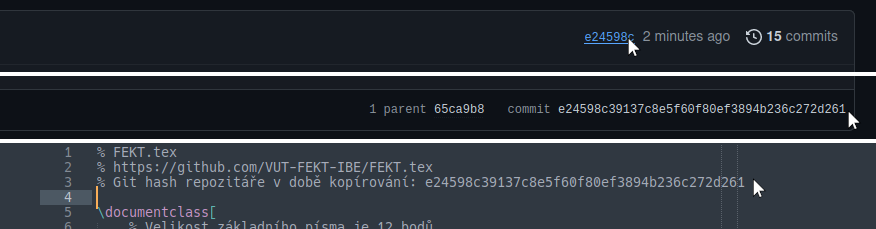
\includegraphics[width=\textwidth]{images/github-commit-hash}
    \caption{Ukázka zkopírování git hashe repozitáře na~GitHub.com}
    \label{img:github-commit-hash}
\end{figure}
\end{verbatim}

\vspace*{1em}

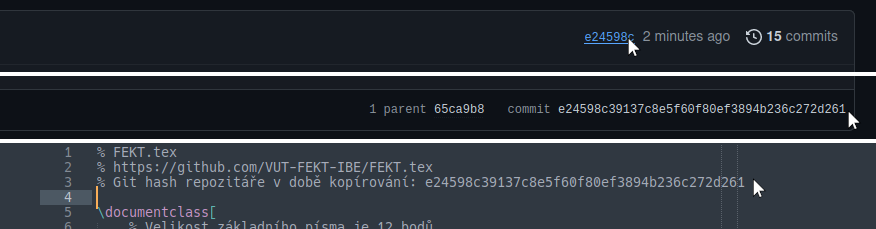
\includegraphics[width=\textwidth]{images/github-commit-hash}
\caption{Ukázka zkopírování git hashe repozitáře na~GitHub.com}
\label{img:github-commit-hash}
\end{mdframed}
\end{figure}
\FloatBarrier

\subsection{O~plovoucích prostředích}

\LaTeX{} většinou nesází obrázek či tabulku přímo v~místě kde ji definujete.
Pokud je objekt plovoucího prostředí (obrázek, tabulka) moc velký a~na~dané místo by vysázen být nemohl, je umístěn na~jiné vhodné místo.

Od~toho slouží nepovinné argumenty které plovoucí prostředí mají:
\\
\verb|\begin{table}[ht]|

Písmena znamenají typ umístění -- \LaTeX{} vybere to nejvhodnější z~nich.

\begin{table}[ht]
    \centering
    \begin{tabular}{|l|l|}
    \texttt{h} & \emph{Here}, místo kde je prostředí definováno \\
    \texttt{t} & \emph{Top}, nejbližší horní strana \\
    \texttt{b} & \emph{Bottom}, nejbližší spodní strana \\
    \texttt{p} & \emph{Page}, zvláštní strana jen pro~plovoucí objekty \\
    \end{tabular}
\end{table}
\FloatBarrier

Volba \texttt{h} sama o~sobě bývá tak špatná, že je automaticky \LaTeX{}em nahrazována volbou \texttt{ht}.
Pokaždé když se začne sázet nová strana, jsou vyprázdněny zásobníky plovoucích prostředí, a~až po~nich je sázen text.

Pokud výchozí chování vypadá špatně a~plovoucí objekt je vysázen nevhodně, můžete za~tabulku umístit příkaz \verb|\FloatBarrier| (z~balíčku \texttt{placeins}) -- ten vynutí vyprázdnění všech zásobníků než se začne sázet text.

Toho využívá i~tento dokument; ukázkové tabulky jsou tak vždy vysázeny dřív než text který s~nimi už nesouvisí.
Pro~delší texty výchozí chování není problematické a~naopak pomáhá udržet konzistenci textu.
Zde jsou však obsaženy spíš kratší odstavce které spolu přímo nesouvisí, a~tabulka, která opožděně skáče do~nového nezávislého textu, ruší pozornost čtenáře.


\end{document}
